% ====================================================================
% VİZE RAPOR ŞABLONU – Türk Masalları Derlemesi Web Sayfası
% --------------------------------------------------------------------
% DERLEME: Overleaf'te Menu > Compiler > XeLaTeX (pdfLaTeX de çalışır).
%
% KURALLAR (şablonu kullanmadan önce okuyun):
%  1. Bölüm başlıklarını SİLMEYİN ve sırasını DEĞİŞTİRMEYİN.
%  2. [KÖŞELİ PARANTEZ] içindeki ve gri renkli açıklama metinlerini
%     kendi bilgilerinizle değiştirin; açıklama metinlerini silin.
%  3. MEBİS'e YALNIZCA bu raporun PDF'ini yükleyin.
%     ZIP ve HTML dosyası YÜKLEMEYİN. Tüm kontroller GitHub'dan yapılır.
%  4. Kapaktaki GitHub ve YouTube bağlantıları doğru ve tıklanabilir
%     olmalıdır. Teslimden önce PDF'teki bağlantılara tıklayıp deneyin.
%  5. Haftalık katkı tablosundaki görseller için resim dosyalarını
%     (hafta1.png, hafta2.png, ...) Overleaf projesine yükleyin.
%     Dosya adlarında boşluk ve Türkçe karakter kullanmayın.
%     Resim yoksa tabloda "görsel ekleyin" kutusu görünür.
%  6. Yapay zekâ kullandıysanız Bölüm 5'i doldurun.
% ====================================================================
\documentclass[12pt,a4paper]{article}

\usepackage{iftex}
\ifPDFTeX
  \usepackage[T1]{fontenc}
  \usepackage[utf8]{inputenc}
\else
  \usepackage{fontspec}
\fi
\usepackage[turkish]{babel}
\usepackage[margin=2.4cm]{geometry}
\usepackage{setspace}
\usepackage{graphicx}
\usepackage{booktabs}
\usepackage{longtable}
\usepackage{array}
\usepackage{colortbl}
\usepackage{xcolor}
\usepackage{enumitem}
\usepackage{listings}
\usepackage{amssymb}
\usepackage{caption}
\usepackage{fancyhdr}
\usepackage{hyperref}

\onehalfspacing
\setlength{\parindent}{0pt}
\setlength{\parskip}{6pt}
\setlist{itemsep=2pt, topsep=4pt}
\hypersetup{colorlinks=true, linkcolor=blue!50!black, urlcolor=blue!50!black}

\definecolor{ana}{HTML}{14325C}
\definecolor{acik}{HTML}{EEF2F8}

\lstset{basicstyle=\ttfamily\small, backgroundcolor=\color{acik},
  frame=single, rulecolor=\color{ana}, breaklines=true,
  columns=fullflexible, keepspaces=true, showstringspaces=false}

\pagestyle{fancy}
\fancyhf{}
\fancyhead[L]{[Gökten Üç Elma — Türk Masalları Derlemesi Web Sayfası]}
\fancyhead[R]{Vize Raporu}
\fancyfoot[C]{\thepage}

% ---------- Yardımcı komutlar ----------
% Gri açıklama metni (silinecek yönergeler için)
\newcommand{\aciklama}[1]{{\color{gray}\itshape (#1)}}

% Haftalık tablo görseli: dosya yoksa "görsel ekleyin" kutusu çıkar
\newcommand{\haftagorsel}[1]{%
  \IfFileExists{#1}{%
    \includegraphics[width=\linewidth,height=4.2cm,keepaspectratio]{#1}%
  }{%
    \fbox{\parbox[c][2.6cm][c]{\dimexpr\linewidth-2\fboxsep-2\fboxrule\relax}{%
      \centering\small\color{gray} Ekran görüntüsü / görsel ekleyin\\ \texttt{#1}}}%
  }%
}
% Haftalık katılım kutuları (işaretlemek için $\square$ yerine $\boxtimes$ yazın)
\newcommand{\katilimkutulari}{\par\vspace{3pt}\small $\square$ Ders içinde katılım sergiledim\par $\square$ Telafi yaptım}

% Ek görsel: dosya yoksa hiçbir şey göstermez
\newcommand{\haftaek}[1]{%
  \IfFileExists{#1}{\\[4pt]\includegraphics[width=\linewidth,height=4.2cm,keepaspectratio]{#1}}{}%
}

% ---------- Kapak bilgileri ----------
\newcommand{\universite}{[ÜNİVERSİTE / BÖLÜM]}
\newcommand{\dersadi}{[DERS ADI]}
\newcommand{\hocaadi}{[ÖĞRETİM ÜYESİ]}
\newcommand{\ogrenciadi}{[AD SOYAD]}
\newcommand{\ogrencino}{[ÖĞRENCİ NUMARASI]}
\newcommand{\projeadi}{[PROJE ADI]}
% Bağlantıları tam adres olarak yazın (https:// ile başlayarak)
\newcommand{\githublink}{\url{https://github.com/KULLANICI-ADI/DEPO-ADI}}
\newcommand{\youtubelink}{\url{https://www.youtube.com/watch?v=VIDEO-KIMLIGI}}
\usepackage{float}
\begin{document} 

% ====================================================================
% KAPAK
% ====================================================================
\begin{titlepage}
\centering
\vspace*{1cm}
{\large \ İstanbul Medipol Üniversitesi/Görsel İletişim Tasarım Bölümü\par}
\vspace{1.8cm}
{\Huge\bfseries\color{ana} \ Gökten Üç Elma \par}
\vspace{0.4cm}
{\Large Türk Masalları Derlemesi Web Sayfası \par}
{\large Vize Raporu \par}
\vspace{1.8cm}
{\large \textbf{Ders:} \ Programlamaya Giriş \par}
{\large \textbf{Öğretim Üyesi:} \ Meral Şentürk \par}
\vspace{1.2cm}
{\large \textbf{Hazırlayan:} \ Selin Naz Gül \par}
{\large \textbf{Öğrenci No:} \ 86250015 \par}
\vspace{1.8cm}
\fbox{\parbox{0.88\linewidth}{\centering\vspace{6pt}
{\large\bfseries Proje Bağlantıları}\\[8pt]
\textbf{GitHub deposu:} https://github.com/selinnazgul/V-ZE-DEV.git \\[8pt]
\textbf{YouTube sunum videosu:} https://youtu.be/eAUcpB4Nyiw
\vspace{6pt}}}
\vfill
{\large \today \par}
\end{titlepage}

\tableofcontents
\newpage

% ====================================================================
\section{Giriş}
% ====================================================================
Projenin amacı, Türk masallarının kısa özetlerini dijital ortamda bir araya getirerek kolay ulaşılabilir ve rahat okunabilir bir web sayfası hazırlamaktır. Bu amaçla “Gökten Üç Elma” adlı bir masal sitesi oluşturulmuştur. Sitede on Türk masalının özetine yer verilmiştir. Kullanıcıların arama özelliğiyle istedikleri masala ulaşmaları ve özetini okuyarak masalın konusu hakkında bilgi edinmeleri amaçlanmıştır. Sayfanın yapısı HTML ile oluşturulmuş, renkleri ve yerleşimi CSS ile düzenlenmiştir. Tasarım kodları içsel CSS, etkileşimli özellikler ise içsel JavaScript olarak aynı HTML dosyasında bir araya getirilmiştir. Bu raporda masalların seçimi, tasarım kararları, kodların çalışma mantığı ve proje geliştirme süreci açıklanmaktadır.

\subsection{Proje Özeti}
Gökten Üç Elma, on Türk masalının kısa özetlerini bir araya getiren bir web sayfasıdır. Kullanıcılar masal adlarını aratarak istedikleri masala ulaşabilir ve özetini okuyabilir. Masalsı bir orman görseli, sıcak renkler ve sade bir düzen kullanılarak kolay anlaşılır ve keyifli bir okuma ortamı oluşturulması amaçlanmıştır.

\subsection{Gereksinimlerin Karşılanması}
\begin{center}
\rowcolors{2}{acik}{white}
\begin{tabular}{@{}p{8.2cm}c@{}}
\toprule
\rowcolor{ana}\textcolor{white}{\textbf{Gereksinim}} & \textcolor{white}{\textbf{Durum}} \\
\midrule
Masal sayısı 8--12 arasında (10 masal)         & $\boxtimes$ \\
Tek HTML dosyası                                    & $\boxtimes$ \\
Stil kodları içsel (\texttt{<style>} içinde)        & $\boxtimes$ \\
Betik kodları içsel (\texttt{<script>} içinde)      & $\boxtimes$ \\
İnternetsiz açılıp çalışıyor                        & $\boxtimes$ \\
JavaScript sayfada anlamlı bir işlev görüyor        & $\boxtimes$ \\
Masal metinleri kendi cümlelerimle yazıldı          & $\square$ \\
Sayfa telefonda da düzgün görünüyor                 & $\boxtimes$ \\
\bottomrule
\end{tabular}
\end{center}

% ====================================================================
\section{Masalların Seçimi}
% ====================================================================
Masalların seçimine, önceden bildiğim birkaç masalı ekleyerek başladım. Ardından farklı Türk masallarını araştırarak derlemeyi on masala tamamladım. Araştırma sırasında konusu ilgimi çeken ve kısa bir özetle anlaşılır biçimde aktarılabilecek masalları tercih ettim. Böylece hem bildiğim hem de bu proje sürecinde tanıdığım masalları bir araya getirdim.

\begin{longtable}{@{}cp{4cm}p{3cm}p{5.4cm}@{}}
\toprule
\textbf{No} & \textbf{Masal} & \textbf{Tür} & \textbf{Seçilme nedeni} \\
\midrule
\endhead
1 & Zümrüdüanka Kuşu & Olağanüstü masal & Araştırma sırasında karşıma çıkması ve konusunu ilgi çekici bulmam. \\
2 & Keloğlan ile Dev & Olağanüstü masal & Keloğlan masallarından farklı bir örneğe yer vermek istemem. \\
3 & Üç Turunçlar & Olağanüstü masal & Daha önce bilmediğim bir masalı araştırarak tanımak istemem. \\
4 & Sabır Taşı & Olağanüstü masal & Araştırırken adına rastlamam ve konusunu merak etmem. \\
5 & Mercan Kız & Olağanüstü masal & Daha önceden bildiğim bir masal olduğu için derlemeye eklemek istemem. \\
6 & Açıl Sofram Açıl & Olağanüstü masal & Araştırma sırasında bulduğum masalın sihirli sofra fikrini ilginç bulmam. \\
7 & Altın Bülbül & Olağanüstü masal & Daha önceden bildiğim ve derlemede bulunmasını istediğim masallardan biri olması. \\
8 & Tuzun Değeri & Gerçekçi masal & Araştırırken bulmam ve günlük yaşamla bağlantılı konusunu beğenmem. \\
9 & Keloğlan ile Padişahın Kızı & Halk masalı & Önceden bildiğim bir Keloğlan masalı olduğu için seçmem. \\
10 & Altın Perçemli Çocukla Sırma Saçlı Kız & Olağanüstü masal & Araştırma sırasında adının dikkatimi çekmesi. \\
\bottomrule
\end{longtable}

% ====================================================================
\section{Tasarım Kararları}
% ====================================================================
Sayfanın tasarımında, kullanıcıların masal özetlerine kolayca ulaşabileceği sade ve anlaşılır bir düzen oluşturulmuştur. Masallar ayrı kartlar içinde sunulmuş, her karta “Özeti Oku” butonu eklenmiştir. Bu düzen sayesinde masal adlarının birbirinden kolayca ayırt edilmesi ve kullanıcının ilgisini çeken içeriği seçebilmesi amaçlanmıştır. Arama alanı ile kullanıcıların bütün kartları tek tek incelemeden istedikleri masalı daha hızlı bulabilmesi sağlanmıştır. Krem zemin ve bordo başlıklar kullanılarak hem sıcak bir görünüm elde edilmesi hem de metinlerin belirgin olması hedeflenmiştir. Kartlarda ve butonlarda aynı renklerin ve benzer biçimlerin tekrarlanmasıyla sayfa genelinde görsel tutarlılık oluşturulmuştur. Kapakta kullanılan masalsı orman görseli ve üç elma motifiyle sitenin adı ve içeriği arasında görsel bir bağlantı kurulmuştur. Süslemelerin içeriğin önüne geçmemesine dikkat edilerek masal özetlerinin ön planda olduğu, kolay kullanılabilir bir arayüz tasarlanmıştır.

\subsection{Konuya Uygunluk}
Tasarımda kullanılan krem ve bordo tonlarıyla, masal kitaplarını çağrıştıran sıcak ve davetkâr bir atmosfer oluşturulması amaçlanmıştır. Krem zemin, metinlerin rahat okunmasını desteklerken bordo başlıklar ve butonlar önemli alanları belirginleştirmek için tercih edilmiştir. Kitap sayfasını anımsatan serifli yazı karakteriyle masalların geleneksel anlatımına uygun bir görünüm hedeflenmiştir. Kapaktaki orman, elma ağacı ve mantar ev, masallardaki hayalî dünyayı yansıtmaktadır. Havada süzülen üç kırmızı elma ise Türk masallarının sonunda kullanılan “Gökten üç elma düşmüş” ifadesine gönderme yaparak sitenin adıyla görsel bir bağ kurmaktadır.

\subsection{Renk Paleti ve Yazı Tipi}
\begin{center}
\rowcolors{2}{acik}{white}
\begin{tabular}{@{}llp{6.4cm}@{}}
\toprule
\rowcolor{ana}\textcolor{white}{\textbf{Ad}} & \textcolor{white}{\textbf{Kod}} & \textcolor{white}{\textbf{Nerede / neden kullandınız?}} \\
\midrule
\relax Bordo & \texttt{[\#7A263A]} & Başlık ve butonları belirginleştirmek, sıcak bir görünüm oluşturmak için kullanılmıştır. \\
\relax Açık Krem & \texttt{[\#FAF3E8]} & Ana zeminde sade ve rahat okunabilir bir görünüm sağlamak için kullanılmıştır. \\
\relax Koyu Krem & \texttt{[\#EBDAC3]} & Gezinme menüsünü ana zeminden ayırmak için kullanılmıştır. \\
\relax Georgia & -- & Kitap sayfasını çağrıştıran serifli yapısı ve okunabilirliği nedeniyle tercih edilmiştir. \\
\bottomrule
\end{tabular}
\end{center}

\subsection{Okunabilirlik, Gezinme ve Duyarlı Tasarım}
\begin{itemize}
  \item \textbf{Okunabilirlik:} Açık krem zemin üzerinde koyu renkli metinler kullanılarak yazıların kolay okunması amaçlanmıştır. Georgia yazı tipi ve geniş satır aralıklarıyla rahat bir okuma düzeni oluşturulmuştur. Başlıklar, boyut ve renk farkıyla metinlerden ayrılarak içerik sırası belirginleştirilmiştir. Metin alanının genişliği sınırlandırılarak satırların fazla uzaması önlenmiş, özetlerin çevresinde boşluk bırakılarak sıkışık bir görünümden kaçınılmıştır.
  \item \textbf{Gezinme:} Kullanıcılar masal kartlarından veya arama alanından istedikleri masala ulaşabilmektedir. Kartlardaki “Özeti Oku” butonları ilgili masalın özetini açmaktadır. “Masallar” ve “Hakkında” menüleriyle bölümler arasında geçiş yapılabilmektedir.
  \item \textbf{Duyarlı tasarım:} Masal kartları geniş ekranlarda yan yana, 600 piksel ve altındaki dar ekranlarda tek sütun hâlinde gösterilecek şekilde düzenlenmiştir. Küçük ekranlarda ana başlığın yazı boyutu azaltılmış, kapak görselinin genişliği ekranı aşmayacak biçimde ayarlanmıştır.
  \item \textbf{Tutarlılık:} Sayfa boyunca aynı renk paleti ve yazı tipi kullanılmıştır. Masal kartlarında benzer boşluklar, yuvarlatılmış köşeler ve aynı biçimde butonlar tercih edilerek bütünlüklü bir görünüm oluşturulmuştur.
\end{itemize}

\subsection{Ekran Görüntüleri}
\begin{figure}[h]
  \centering
\resizebox{0.65\textwidth}{!}{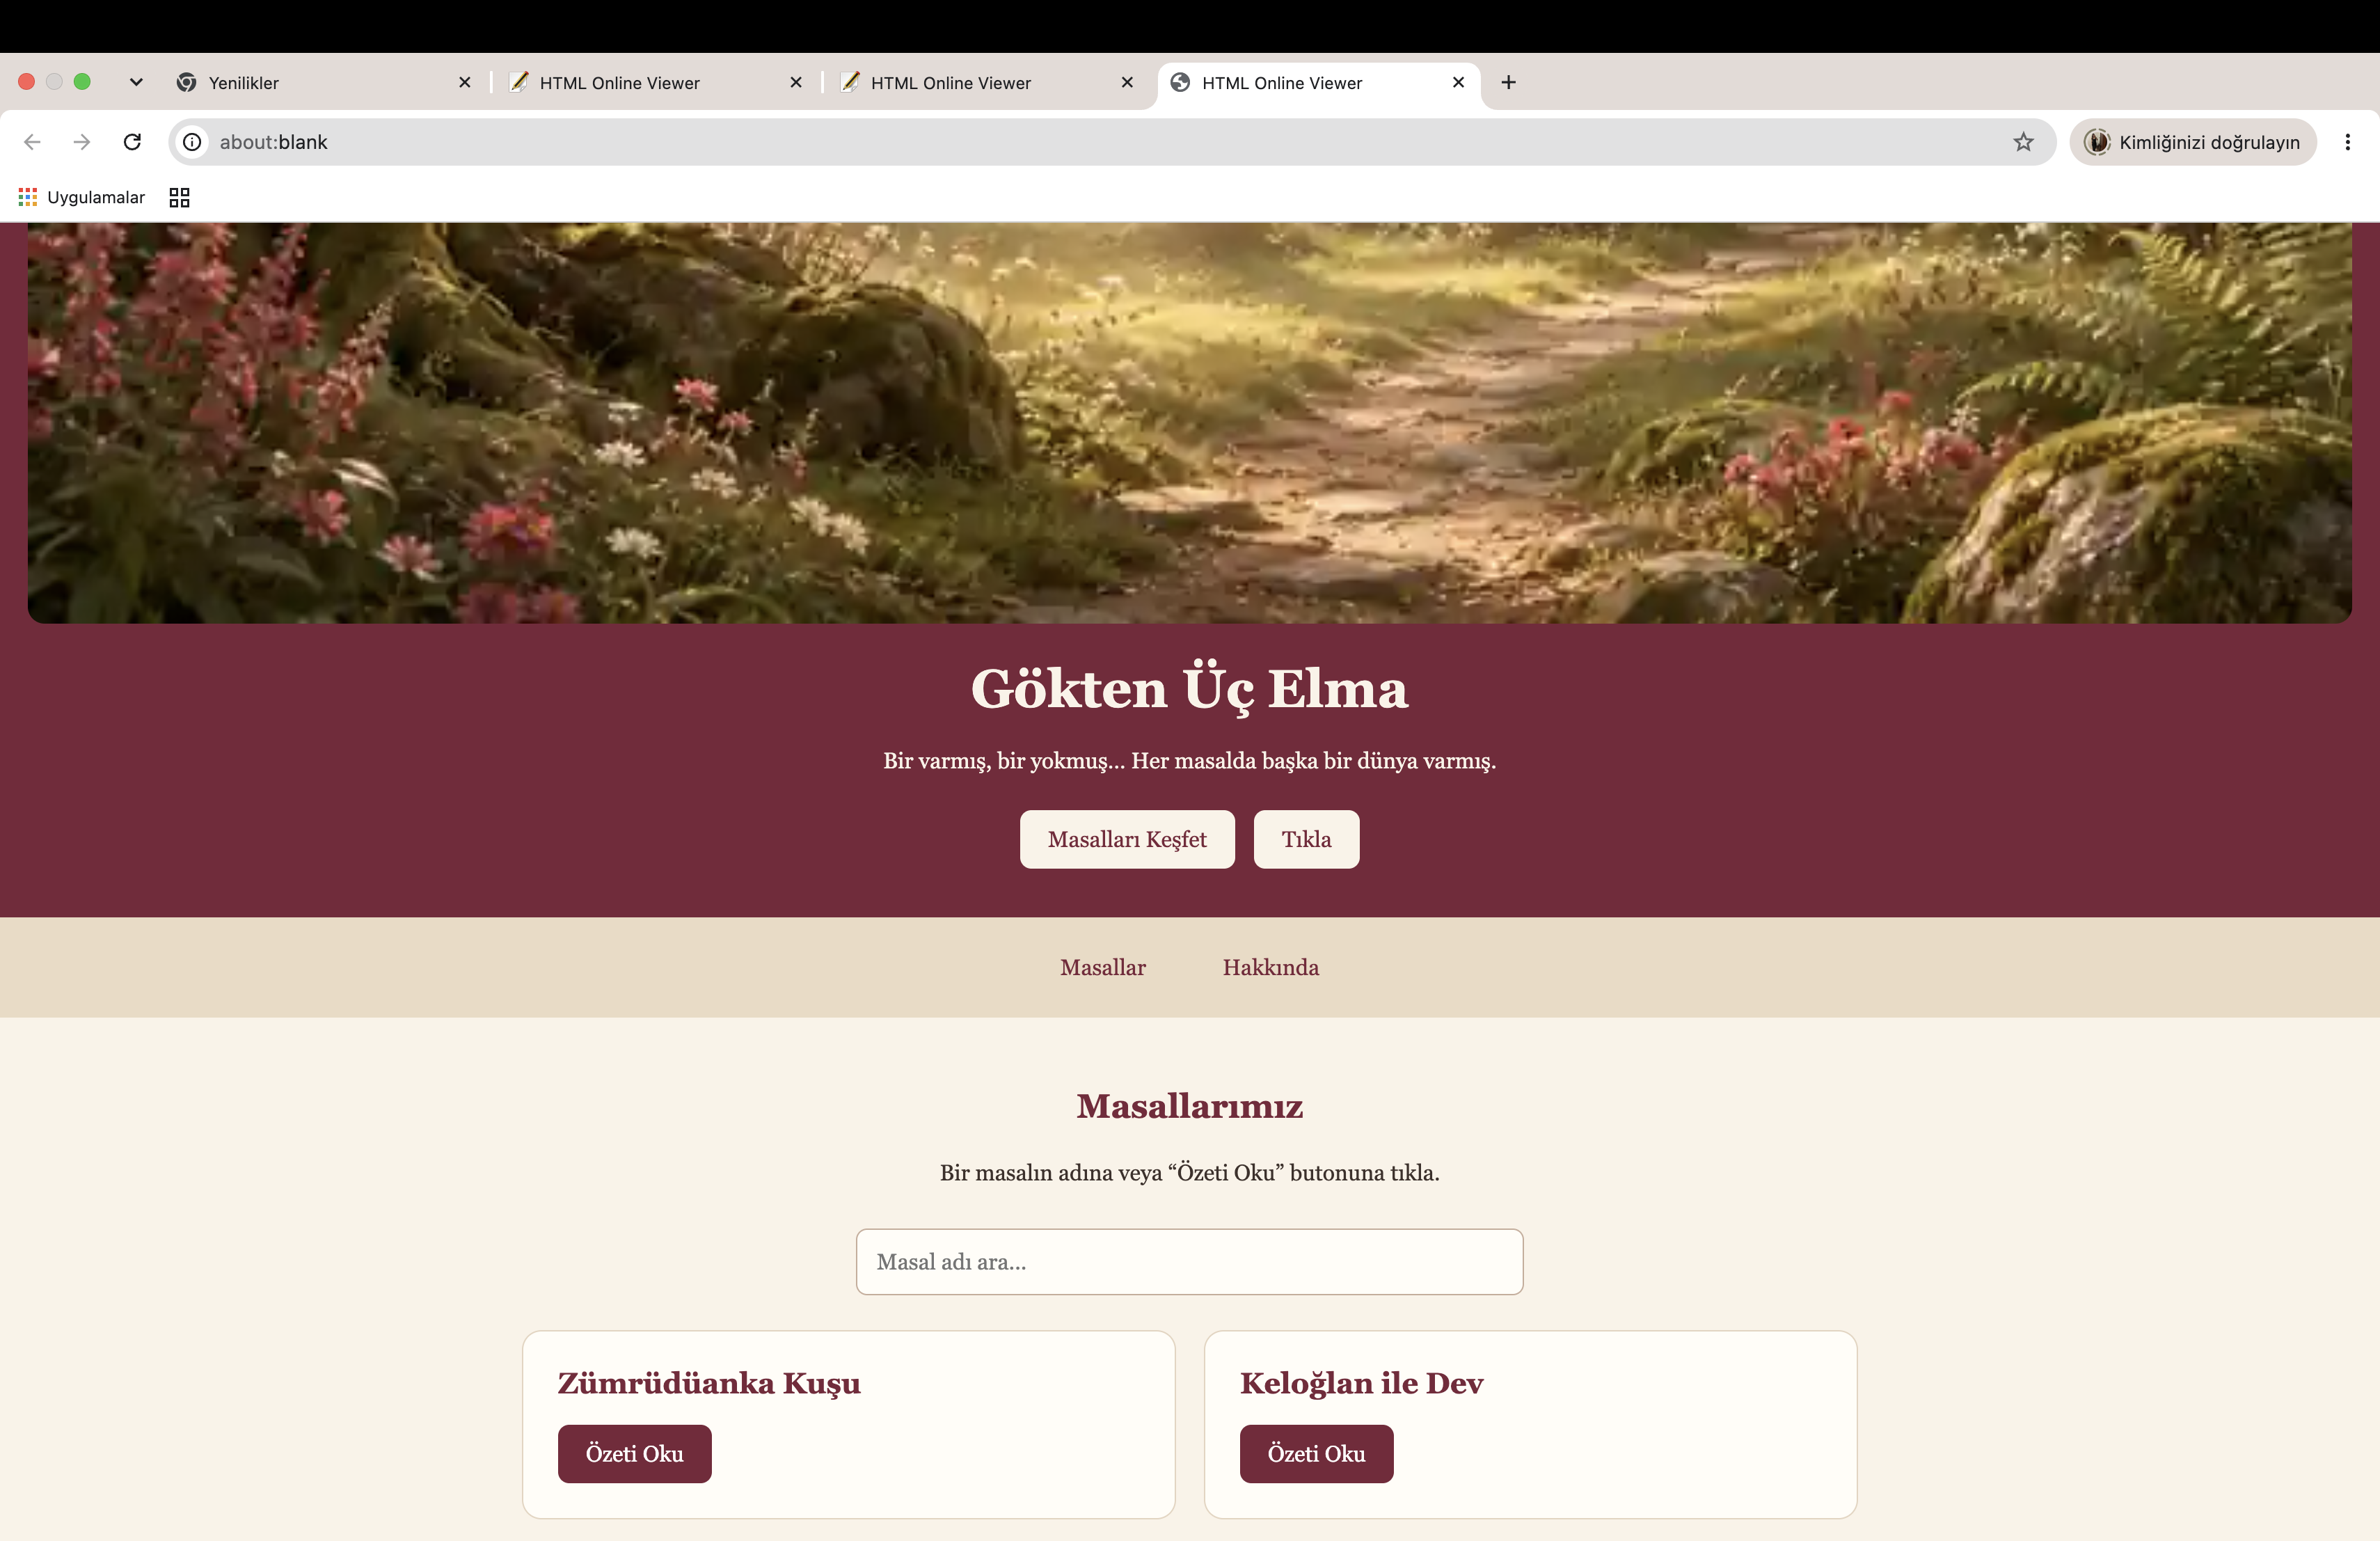
\includegraphics{ekran-masaustu.png}}
  \caption{Sayfanın bilgisayar görünümü}
 \end{figure}
\begin{figure}[H]
  \centering
\resizebox{0.20\textwidth}{!}{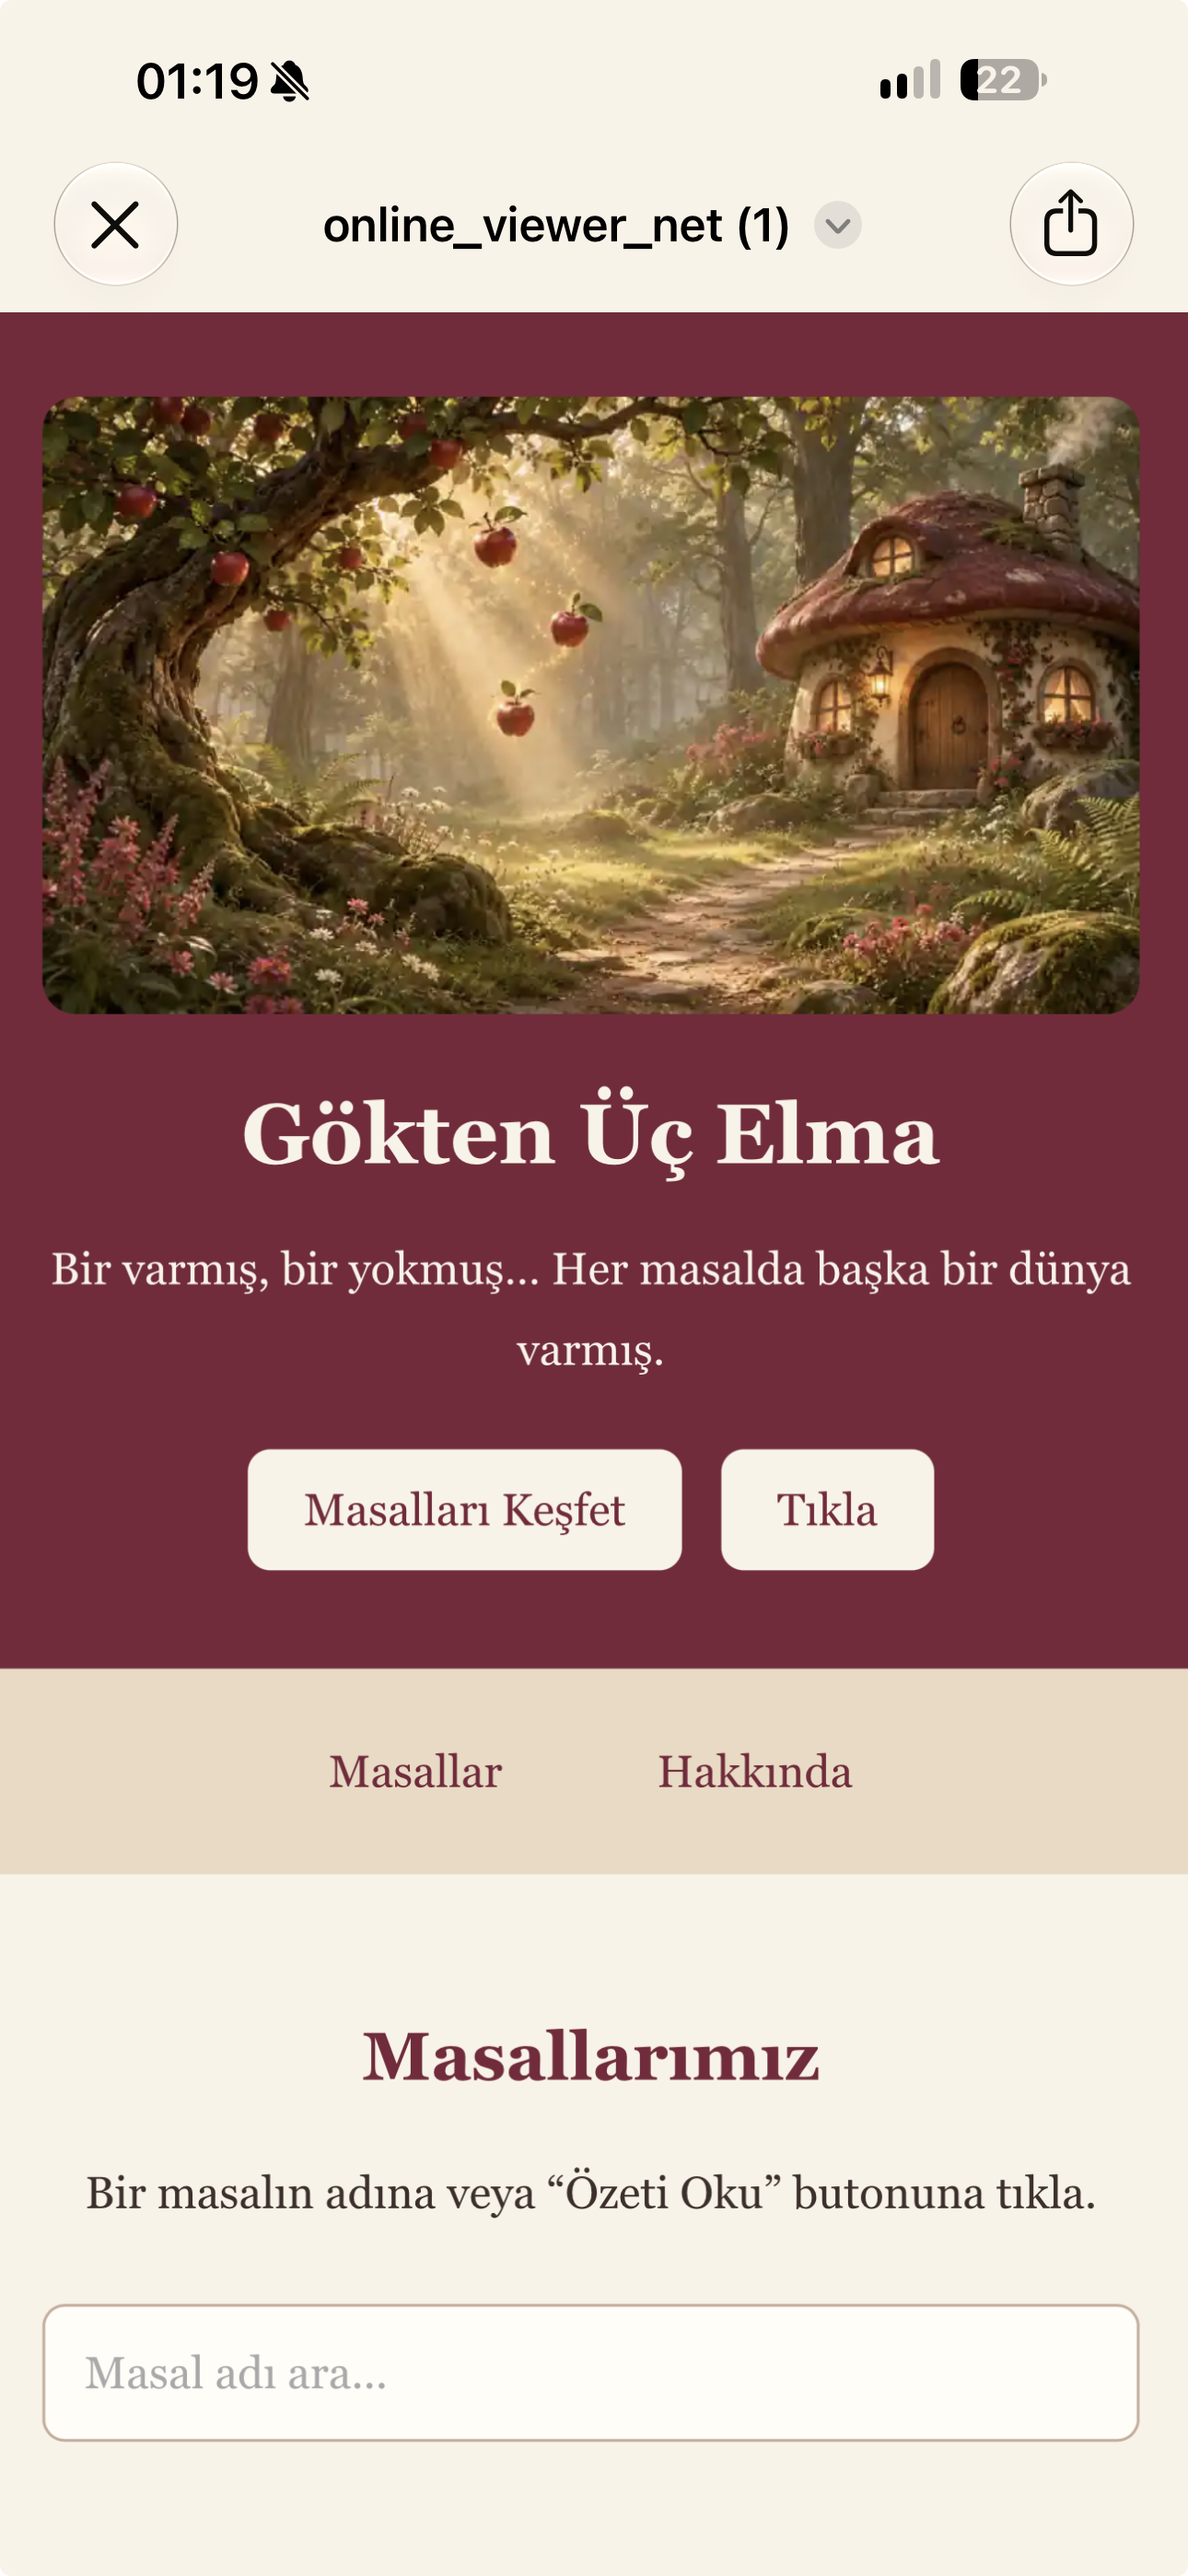
\includegraphics{ekran-mobil.png}}
   \caption{Sayfanın telefon görünümü}
\end{figure}
% ====================================================================
\section{Gerçekleştirme}
% ====================================================================
“Gökten Üç Elma” adlı masal sitesi HTML, CSS ve JavaScript kullanılarak hazırlanmıştır. HTML ile sayfanın temel yapısı oluşturulmuş; başlık, menü, masal kartları ve içerik bölümleri düzenlenmiştir. CSS ile sitenin renkleri, yazı tipleri, boşlukları ve genel görünümü belirlenmiştir. JavaScript ile masalların aranması ve kullanıcıların içerikler arasında gezinmesi sağlanmıştır.

Kullanıcılar ana sayfada bulunan masal kartları üzerinden istedikleri masalı seçerek içeriğine ulaşabilmektedir. Arama özelliği sayesinde masalları daha kolay bulabilmektedir. Ayrıca site, bilgisayar ve telefon ekranlarına uyum sağlayacak şekilde tasarlanmıştır.

\subsection{HTML Yapısı}

\subsection{İçsel CSS}
Masal kartlarını CSS Grid ile iki sütun halinde düzenledim. Ekran genişliği 600 piksel veya daha az olduğunda kartları tek sütuna indirdim ve ana başlığın yazı boyutunu 30 piksele düşürdüm. Böylece site dar ekranlarda daha rahat okunabiliyor.

\begin{lstlisting}[caption={İçsel CSS'ten önemli bir bölüm}]
.masallar {
    display: grid;
    grid-template-columns: repeat(2, minmax(0, 1fr));
    gap: 20px;
    align-items: start;
}

@media (max-width: 600px) {
    .masallar {
        grid-template-columns: 1fr;
    }

    h1 {
        font-size: 30px;
    }
}
\end{lstlisting}

\subsection{İçsel JavaScript}
Masalları HTML dosyasının script bölümünde masallar adlı bir dizide tuttum. Dizideki her nesnenin ad alanında masalın başlığı, ozet alanında ise kısa özeti yer alıyor. JavaScript bu bilgilerle her masal için bir kart oluşturuyor. Masal başlığına ve “Özeti Oku” düğmesine addEventListener ile tıklama olayı bağladım. İkisine de tıklandığında ozetAc() fonksiyonu özeti açıp kapatıyor. Kullanıcı arama kutusunda yazı yazdığında veya sildiğinde oninput olayı masalAra() fonksiyonunu çalıştırıyor. Bu fonksiyon eşleşmeyen kartları gizliyor ve hiç eşleşme yoksa “Aradığın masal bulunamadı.” mesajını gösteriyor. bolumAc() fonksiyonu ise Masallar ve Hakkında bölümleri arasında geçiş yapıyor.

\begin{lstlisting}
function masalAra() {
    const aranan = document.getElementById("arama").value
        .trim().toLocaleLowerCase("tr-TR");

    const kartlar = document.querySelectorAll(".kart");
    let bulunan = 0;

    kartlar.forEach(function(kart) {
        const ad = kart.querySelector("h3").textContent
            .toLocaleLowerCase("tr-TR");

        const eslesiyor = ad.includes(aranan);
        kart.hidden = !eslesiyor;

        if (eslesiyor) {
            bulunan++;
        }
    });

    document.getElementById("sonucYok").hidden = bulunan > 0;
}
\end{lstlisting}

\subsection{Sayfanın Özellikleri}


% ====================================================================
\section{Yapay Zekâ Kullanımı}
% ====================================================================
ChatGPT’yi, kod yazarken takıldığım bölümlerde destek almak ve Gökten Üç Elma sitesinin kapak görselini oluşturmak için kullandım.

\begin{longtable}{@{}p{2.6cm}p{3.6cm}p{4.2cm}p{3.4cm}@{}}
\toprule
\textbf [Araç adı]& \textbf{Ne için kullandınız?} & \textbf{İstem (prompt) özeti} & \textbf{Sayfada nerede?} \\
\midrule
\endhead
\relax ChatGBT & Kapak görseli üretmek için. & Mantar ev ve üç elmanın bulunduğu masalsı bir orman görseli oluştur. & Ana sayfanın üstündeki kapak görseli \\
\relax ChatGBT & JavaScript arama kodunu anlamak için. & Yazılan kelimeye göre masal kartlarının nasıl filtrelendiğini açıkla. & Masallar bölümündeki arama kutusu \\
\relax ChatGBT & Kod yazarken takıldığım bölümleri tamamlamak için. & Mevcut HTML dosyama uygun şekilde, yazmakta zorlandığım kısımlar için kısa kod örnekleri ver. & Sayfanın farklı bölümlerindeki kod parçalarında. \\
\bottomrule
\end{longtable}

\subsection{Anladığım ve Kendim Yaptığım Kısımlar}
Kod yazarken takıldığım yerlerde ChatGPT’den destek aldım. Arama kodunu incelerken, arama kutusuna yazdığım metnin masal başlıklarıyla karşılaştırıldığını ve eşleşmeyen kartların gizlendiğini anladım. Sitenin masaüstü ve mobil görünümlerini karşılaştırarak kartların dar ekranda iki sütundan tek sütuna geçtiğini kontrol ettim. JavaScript örneğini rapora eklerken fonksiyonun ilk satırı PDF’de görünmedi. Fonksiyon başlığını yeni satıra alarak kod örneğinin tamamının görünmesini sağladım.

% ====================================================================
\section{Haftalık Katkılar}
% ====================================================================
\aciklama{Her hafta ders içinde yaptığınız çalışmayı kısaca yazın (2--4 cümle). Hangi
özelliği eklediğinizi ya da neyi düzelttiğinizi belirtin ve ilgili commit mesajını
ya da bağlantısını ``Commit'' satırına yazın. Her satıra ekran görüntüsü ekleyin:
resimleri \texttt{hafta1.png}, \texttt{hafta2.png}, \ldots{} adıyla Overleaf
projesine yükleyin. Aynı haftaya ikinci bir görsel eklemek için
\texttt{hafta1b.png} gibi bir dosya yükleyin; kendiliğinden görünür.
Her haftanın altındaki kutulardan o hafta için geçerli olanı $\boxtimes$ ile
işaretleyin: dersin kendisinde katılım gösterdiyseniz ``Ders içinde katılım
sergiledim'', o haftayı sonradan tamamladıysanız ``Telafi yaptım''. Telafi
yaptıysanız yapılan çalışmanın metninde bunu açıkça belirtin.}

\begin{longtable}{@{}>{\raggedright\arraybackslash}p{1.7cm}%
                    >{\raggedright\arraybackslash}p{6.4cm}%
                    >{\centering\arraybackslash}p{6cm}@{}}
\toprule
\rowcolor{ana}\textcolor{white}{\textbf{Hafta}} & \textcolor{white}{\textbf{Yapılan çalışma}} & \textcolor{white}{\textbf{Görsel}} \\
\midrule
\endfirsthead
\toprule
\rowcolor{ana}\textcolor{white}{\textbf{Hafta}} & \textcolor{white}{\textbf{Yapılan çalışma}} & \textcolor{white}{\textbf{Görsel}} \\
\midrule
\endhead
\bottomrule
\endfoot

\textbf{1. hafta}\newline 23 Eylül 2026 &
WorldWideWeb başlıklı sayfa üzerinde temel HTML yapısı çalışıldı. Başlık, paragraf, liste ve bağlantılar kullanılarak içerik bölümlere ayrıldı. Sayfa içi bağlantılarla ilgili bölüme ulaşma yaklaşımı incelendi. \newline \textbf{Commit:} Henüz eklenmedi. \newline $\boxtimes$ Ders içinde katılım sergiledim
\newline $\square$ Telafi yaptım & 
\begin{minipage}[t]{\linewidth}
  \vspace{0pt}
  \centering
  \haftagorsel{hafta1.png}\haftaek{hafta1b.png}
\end{minipage} \\
\midrule
\textbf{2. hafta}\newline 30 Eylül 2026 &
“Kiraz Mevsimi” dizisi için bir tanıtım sayfası hazırladım. Sayfada dizinin konusuna, kısa özetine, oyuncularına ve görsellerine yer verdim. Açılır soru alanları ekledim ve tıklama, çift tıklama, fareyle üzerine gelme ve bağlantı açma örnekleri üzerinde çalıştım. \newline \textbf{Commit:} Henüz eklenmedi. 
\newline $\boxtimes$ Ders içinde katılım sergiledim
\newline $\square$ Telafi yaptım &
\begin{minipage}[t]{\linewidth}
  \vspace{0pt}
  \centering
  \haftagorsel{hafta2.png}\haftaek{hafta2b.png}
\end{minipage} \\
\midrule
\textbf{3. hafta}\newline 7 Ekim 2026 &
Kullanıcıdan isim alan bir giriş kutusu ve düğme üzerinde çalışıldı. JavaScript ile giriş alanının değeri alınarak sayfada selamlama metni oluşturma yaklaşımı incelendi. Boş giriş için koşul kullanımı çalışıldı. \newline \textbf{Commit:} Henüz eklenmedi. \newline $\boxtimes$ Ders içinde katılım sergiledim
\newline $\square$ Telafi yaptım &
\begin{minipage}[t]{\linewidth}
  \vspace{0pt}
  \centering
  \haftagorsel{hafta3.png}\haftaek{hafta3b.png}
\end{minipage} \\
\midrule
\textbf{4. hafta}\newline 14 Ekim 2026 &
Bağlantı ve düğme ile farklı sayfalara yönlendirme çalışıldı. Renk eşleştirme örneğinde kartların veri özellikleri okundu ve aynı ya da farklı renklerin nasıl karşılaştırıldığı incelendi. Zamanlayıcı ve sınıf ekleme işlemleri kullanıldı. \newline \textbf{Commit:} Henüz eklenmedi. \newline $\boxtimes$ Ders içinde katılım sergiledim
\newline $\square$ Telafi yaptım &
\begin{minipage}[t]{\linewidth}
  \vspace{0pt}
  \centering
  \haftagorsel{hafta4.png}\haftaek{hafta4b.png}
\end{minipage} \\
\midrule
\textbf{5. hafta}\newline 21 Ekim 2026 &
Bu haftanın çalışmasını sonradan telafi ettim. Harici CSS dosyasını HTML’e bağlama ve Bootstrap sınıflarıyla başlık, gezinme, bölüm ve kart düzeni oluşturma üzerine çalıştım. Düğmeye tıklandığında bir kutunun rengini değiştiren örneği de uyguladım. \newline \textbf{Commit:} Henüz eklenmedi. \newline $\square$ Ders içinde katılım sergiledim
\newline $\boxtimes$ Telafi yaptım &
\begin{minipage}[t]{\linewidth}
  \vspace{0pt}
  \centering
  \haftagorsel{hafta5.png}\haftaek{hafta5b.png}
\end{minipage} \\
\end{longtable}
% ====================================================================
\section{Test ve Değerlendirme}
% ====================================================================
Gökten Üç Elma sitesini MacBook bilgisayarımda ve iPhone telefonumda denedim. Testlerde Safari ve Google Chrome tarayıcılarını kullandım. “Masalları Keşfet” ve “Masallar” düğmeleri masal listesine, “Hakkında” düğmesi ise Hakkında bölümüne yönlendirdi. “Tıkla” düğmesine bastığımda MacBook’ta “Gökten Üç Elma’ya hoş geldin” mesajı göründü, ancak iPhone’da mesaj görünmedi. Bu farkın nedenini henüz belirleyemedim.

\begin{center}
\rowcolors{2}{acik}{white}
\begin{tabular}{@{}p{6cm}p{3.4cm}p{3.4cm}@{}}
\toprule
\rowcolor{ana}\textcolor{white}{\textbf{Özellik}} & \textcolor{white}{\textbf{Bilgisayar}} & \textcolor{white}{\textbf{Telefon}} \\
\midrule
\relax Masalları Keşfet ve Masallar düğmeleriyle masal listesine gitme & Çalışıyor & Çalışıyor \\
\relax Hakkında düğmesiyle Hakkında bölümüne gitme & Çalışıyor & Çalışıyor \\
\relax Tıkla düğmesiyle karşılama mesajını gösterme & Çalışıyor & Sorun var \\
\relax Masal adına göre arama & Çalışıyor & Çalışıyor \\
\relax Özeti Oku ve Özeti Kapat düğmeleriyle özeti açıp kapatma & Çalışıyor & Çalışıyor \\
\bottomrule
\end{tabular}
\end{center}

\textbf{Denenen tarayıcılar:} Chrome, Safari

% ====================================================================
\section{Sunum Videosu}
% ====================================================================
\begin{flushleft}
\begin{tabular}{@{}ll@{}}
\textbf{Video süresi:} & 15:09 \quad \\
\textbf{Görünürlük:} & Listelenmemiş \\
\textbf{Bağlantı:} & https://youtu.be/eAUcpB4Nyiw \\
\end{tabular}
\end{flushleft}

\subsection{Video Kontrol Listesi}
\aciklama{Teslimden önce hepsini kontrol edin ve kutuları $\boxtimes$ ile işaretleyin.}
\begin{itemize}
  \item $\boxtimes$ Süre 12--18 dakika aralığında.
  \item $\boxtimes$ Sunum boyunca kameram açık, yüzüm görünüyor.
  \item $\boxtimes$ Görünürlük \textbf{Listelenmemiş} (ya da Herkese açık); \textbf{Özel} değil.
  \item $\boxtimes$ Bağlantıyı gizli pencerede açtım, video oynuyor.
  \item $\boxtimes$ YouTube videoyu işlemeyi bitirdi.
  \item $\boxtimes$ Videoyu baştan sona izledim; ses ve kamera tüm sunumda var.
  \item $\boxtimes$ Kapaktaki bağlantı ile bu bölümdeki bağlantı aynı.
\end{itemize}

% ====================================================================
\section{Sonuç ve Kendi Değerlendirmem}
% ====================================================================
Gökten Üç Elma projesinde en çok HTML dosyasını hazırlarken ve kod yazarken zorlandım. Takıldığım yerlerde ChatGPT’den destek aldım. Verdiği örnekler ve açıklamalar, bazı kod satırlarının ne işe yaradığını anlamama yardımcı oldu. Mesela arama kutusuna yazılan kelimenin masal başlıklarıyla karşılaştırıldığını ve eşleşmeyen kartların gizlendiğini kodda takip edebildim. Siteyi MacBook ve iPhone’da denerken “Tıkla” düğmesinin karşılama mesajını bilgisayarda gösterdiğini, telefonda ise mesajın görünmediğini fark ettim. İleride bunun nedenini bulup düğmenin telefonda da çalışmasını sağlamak isterim.

% ====================================================================
\section{Kaynakça}
% ====================================================================

\begin{thebibliography}{99}

\bibitem{chatgpt}
OpenAI. \emph{ChatGPT}.
\url{https://chatgpt.com/}

\bibitem{zumruduanka}
Masal Sitesi. \emph{Zümrüdüanka Kuşu Okuma Masalı}.
\url{https://www.masalsitesi.com/Zumruduanka-Kusu-Masali.html}

\bibitem{keloglandev}
Masal.org. \emph{Keloğlan ile Dev Masalı}.
\url{https://www.masal.org/keloglan-ile-dev/}

\bibitem{ucturunclar}
Bilge Baba. \emph{Üç Turunçlar}.
\url{https://bilgebaba.com/uc-turunclar/}

\bibitem{sabirtasi}
T.C. Kültür ve Turizm Bakanlığı, Kültür Portalı.
\emph{Masal Anlatıcılarının Bilinçaltlarında Adalet Kavramı}, Sabır Taşı bölümü.
\url{https://www.kulturportali.gov.tr/Common/DownloadFile.aspx?f=MasalAnlaticilarininBilincaltlarindaAdaletKavrami_20190318110757340.pdf}

\bibitem{mercankiz}
Masalpu. \emph{Mercan Kız Masalı}.
\url{https://masalpu.com/mercan-kiz-masali/}

\bibitem{acilsofram}
Masal Oku. \emph{Açıl Sofram Açıl Masalı}.
\url{https://www.masaloku.net/acil-sofram-acil-masali/}

\bibitem{altinbulbul}
Tekman İlçe Millî Eğitim Müdürlüğü.
\emph{Okuma Saati}, Altın Bülbül bölümü.
\url{https://tekman.meb.gov.tr/meb_iys_dosyalar/2020_03/27204540_dergi_v2.pdf}

\bibitem{tuzundegeri}
Masal.org. \emph{Kıymetli Tuz Masalı}.
\url{https://www.masal.org/kiymetli-tuz/}

\bibitem{keloglanpadisah}
Masalbaz. \emph{Keloğlan ile Padişahın Kızı Masalı}.
\url{https://masalbaz.com/keloglan-ile-padisahin-kizi/}

\bibitem{altinpercemli}
Necmettin Erbakan Üniversitesi Açık Erişim Arşivi.
\emph{Altın Perçemli Çocukla Sırma Saçlı Kız}, bölüm 4.9.
\url{https://acikerisim.erbakan.edu.tr/bitstreams/93481796-ba8c-46f0-84d1-7d7c3f3afb7d/download}

\bibitem{kapakgorseli}
OpenAI. (2026). \emph{Gökten Üç Elma kapak görseli}.
Ana sayfanın kapağında kullanılan görsel ChatGPT ile üretildi.

\end{thebibliography}

% ====================================================================
\appendix
\section{Teslim Kontrol Listesi}
% ====================================================================

\begin{itemize}
  \item $\boxtimes$ MEBİS'e \textbf{yalnızca bu raporun PDF'ini} yükleyeceğim. ZIP ve HTML dosyası yüklemeyeceğim.
  \item $\boxtimes$ PDF dosya adı \texttt{OgrenciNo\_AdSoyad\_vize.pdf} biçiminde.
  \item $\boxtimes$ Kapaktaki GitHub ve YouTube bağlantıları doğru; PDF'te tıklayıp denedim.
  \item $\boxtimes$ GitHub deposunda web sayfası (tek \texttt{.html}), rapor PDF'i, \texttt{.tex} kaynakları ve \texttt{README.md} var.
  \item $\boxtimes$ GitHub deposu \textbf{herkese açık} (ya da öğretim üyesine erişim verdim).
  \item $\boxtimes$ Çalışmamın son hâli teslim saatinden \textbf{önce} depoya gönderildi (sonraki commitler değerlendirilmez).
  \item $\boxtimes$ Sayfa içsel CSS ve içsel JavaScript kullanıyor, harici dosya gerektirmiyor.
  \item $\boxtimes$ Hazır taslak kullanmadım; yapay zekâ kullandıysam Bölüm 5'i doldurdum.
  \item $\boxtimes$ Çalışmanın mantığını sunumda anlatabilirim.
\end{itemize}

\end{document}